\input{lib/packs}

\geometry{left=1cm}% левое поле
\geometry{right=1cm}% правое поле
\geometry{top=1cm}% верхнее поле
\geometry{bottom=2cm}% нижнее поле

%\renewcommand{\baselinestretch}{1.3}

\begin{document}
\input{lib/macro}


\paragraph{Аттрактор, частично лежащий в пространстве траекторий}
\paragraph{}
Пример дифференциального уравнения:
\begin{equation}\label{primer_iz_statyi}
	u'(t)=
	\left\{
		\begin{array}{ll}
			-(u(t)-1)^2, & u(t) > 1, \\
			-u^2 (t)   , & 0 \leq u(t) \leq 1 \\
			u^2 (t)    , & u(t) < 0
		\end{array}
	\right.
\end{equation}

Решение:
\begin{equation}\label{primer_iz_statyi_u_t}
	\left[
		\begin{array}{ll}
			u=\frac{1}{t+C}+1, & C>0
		\\\\
			u=\frac{1}{t+1+C}, & C\geq0
		\\\\
			u=0,               & C \mbox{--- любое}
		\\\\
			u=-\frac{1}{t+C},  & C>0
		\end{array}
	\right.
\end{equation}

Задача Коши однозначно разрешима.

\opred
Оператором сдвига $S^{t_0}_t$ по траекториям дифференциального уравнения $x'(t) = f(x,t)$ называется функция, такая, что
\begin{equation*}
	S^{t_0}_t (p) = q \Rightleftarrow
		\exists\left(x_p(t) : x_p(t_0) = p\right)\left[x_p(t) = q\right].
\end{equation*}

\paragraph{Обозначение.}
$S^{0}_t (p) = S_t (p)$
В случае, если $t_0=0$, соответствующий оператор сдвига по траекториям дифференциального уравнения $S^{t_0}_t (p)$ в целях упрощения записи  в дальнейшем будем обозначать просто $S_t (p)$.

Оператор сдвига по траекториям уравнения (\ref{primer_iz_statyi}) :
\begin{equation}\label{oper_sdviga_primer_1}
	S_t p =
	\left\{
		\begin{array}{ll}
			\frac{p+pt-t}{pt-t+1}, & p > 1
		\\\\
			\frac{p}{pt+1},        & 0 \leq p \leq 1
		\\\\
			\frac{p}{1 - pt},      & p < 0
		\end{array}
	\right.
\end{equation}


\paragraph{Вспомогательные определения.}
\paragraph{~}
$E$ --- рефлексивное банахово пространство, $E_0$ --- банахово пространство, вложение $E \subset E_0$ непрерывно,
$F$ --- топологическое пространство, $E \cap F \ne \varnothing$.

\paragraph{Обозначение.}
$T_+ = C(\mathbb{R}_+,E_0) \cap L_\infty(\mathbb{R}_+,E)$

\opred
Оператором сдвига $T(h)$, $h\in\R$ называется оператор, который функции $f$ ставит в соответствие функцию $T(h)f$, такую, что
$
T(h)f(t)=f(t+h)
$.

\opred
Пространство траекторий $\mathcal{H}^+$ трансляционно инвариантно, если
$
	\forall(t \geq 0)\left[T(t)\mathcal{H}^+ \subset \mathcal{H}^+ \right]
$

\opred

Пусть $B \subset T_+$.
Сечением множества траекторий $B$ в момент времени $t \geq 0$ называется множество
$
	B(t)=\left\{u(t) : u \in B \right\} \subset E.
$


\opred

Пусть $R,Q \subset E$.
Полуотклонением в пространстве $E_0$ множества $R$ от множества $Q$ называется величина
$
	h_{E_0}(R,Q) = \sup_{r\in R} \inf_{q \in Q} \| q - r \|_{E_0}.
$


\paragraph{Аттрактор полугруппы трансляций}

\opred
Семейство отображений $S_t : E \to E$, $t \geq 0$ называется полугруппой трансляций,
если $S_0$ --- тождественное отображение и
$
	\forall(t>0,\tau>0)[S_t \circ S_\tau = S_{t+\tau}]
$

\opred
Полугруппа $S_t$ называется ограниченной в $E$, если для любого ограниченного в $E$ множества
$B \subset E$ множество $\bigcup\limits_{t\geq0}S_t B$ также ограничено в $E$.

\opred

Множество $A$ инвариантно относительно полугруппы трансляций $S_t$, если
$
	\forall(t\geq 0)[S_t A = A]
$

\opred

Множество $P \subset F$ называется $(E,F)$-притягивающим для полугруппы трансляций $S_t$,
если для любого ограниченного множества $B \subset E$ и любой открытой окрестности $W$ множества $P$ в $F$ существует
число $h\geq 0$ такое, что
$
	\forall(t \geq h)[S_t B \subset W]
$


\opred

Множество $A\subset E\cap F$ называется $(E,F)$-аттрактором полугруппы трансляций $S_t$, если

а) $A$ компактно в $F$ и ограничено в $E$;

б) $A$ инвариантно относительно полугруппы трансляций $S_t$.

в) $A$ является $(E,F)$-притягивающим для полугруппы трансляций $S_t$.

\paragraph{Утверждение 1.}
У полугруппы трансляций (\ref{oper_sdviga_primer_1}) нет $(\mathbb{R},\mathbb{R})$-аттрактора.

\paragraph{Минимальный траекторный аттрактор}

\opred

Множество $P \subset T_+$ называется притягивающим для пространства траекторий $\mathcal{H}^+$
в топологии пространства $C(\mathbb{R}_+; E_0)$,
если для всякого множества $B \subset \mathcal{H}^+$, ограниченного в $L_{\infty}(\mathbb{R}_+;E)$, выполняется условие
$
	h_{E_0}(B(t),T(t)P) \xrightarrow[t\to\infty]{}0
$

\opred

Непустое множество $\mathcal{U}\subset T^+$
называется траекторным аттрактором для пространства траекторий $\mathcal{H}^+$
относительно топологии $C(\mathbb{R}_+,E_0)$, если
\begin{enumerate}
	\item)
		$\mathcal{U}$ компактно в $C(\mathbb{R}_+,E_0)$;
	\item)
		$\mathcal{U}$ ограничено в $L_{\infty}(\mathbb{R}_+,E)$;
	\item)
		$\mathcal{U}$ трансляционно инвариантно;
	\item)
		$\mathcal{U}$ является притягивающим для пространства траекторий $\mathcal{H}^+$
		в топологии пространства $C(\mathbb{R}_+; E_0)$.
\end{enumerate}

\opred
Минимальным траекторным аттрактором пространства траекторий $\mathcal{H}^+$
называется такой траекторный аттрактор, который содержится в любом другом траекторном аттракторе.

\paragraph{Утверждение 2.}
Для уравнения (\ref{primer_iz_statyi}) минимальный траекторный аттрактор имеет вид
$
	P = \{ v_0(t) \equiv 0, v_1(t) \equiv 1\}
$

\paragraph{Утверждение 3.}
Функция $v_1(t) \equiv 1$ принадлежит минимальному траекторному аттрактору,
но не принадлежит пространству траекторий.


\paragraph{Глобальный аттрактор}

\opred

Множество  $\mathcal{A} \subset E $ называется глобальным аттрактором (в $E_0$) для пространства траекторий $\mathcal{H}^+$, если:
\begin{enumerate}
	\item)
		$\mathcal{A}$ компактно в $E_0$ и ограничено в $E$;
	\item)
		для любого ограниченного в $L_\infty(\mathbb{R}_+; E)$ множества $X \subset \mathcal{H}^+$
		выполнено условия притягивания
		$$
			h_{E_0}(X(t),\mathcal{A}) \xrightarrow[t\to \infty]{}{0}.
		$$
	\item)
		$\mathcal{A}$ --- наименьшее по включению множество, удовлетворяющее условиям (1) и (2).
\end{enumerate}

\paragraph{Утверждение 4.}
Глобальным аттрактором явлется множество $G = P(t) = \{0; 1\}$.

\paragraph{Минимальный траекторный аттрактор, целиком лежащий вне пространства траекторий}

\paragraph{Второй пример дифференциального уравнения}

Положим $E=E_0=\R^2$.
Разобьём $\R^2$ на пять непересекающихся связных множеств следующим образом:
$$
	A_0 = \{ (x_1, x_2) \mid 0 < x_1 < 1,~~ 0 < x_2 < 1\}
$$
$$
	A_1 = \{ (x_1, x_2) \mid x_1 < 1,~~ x_2 \leq 0  \}
$$
$$
	A_2 = \{ (x_1, x_2) \mid x_1 \geq 1,~~ x_2 < 1  \}
$$
$$
	A_3 = \{ (x_1, x_2) \mid x_1 > 0,~~ x_2 \geq 1  \}
$$
$$
	A_4 = \{ (x_1, x_2) \mid x_1 \leq 0,~~ x_2 > 0  \}
$$

\paragraph{~}
и отметим точки
$\alpha_1=(1, 0)$,
$\alpha_2=(1, 1)$,
$\alpha_3=(0, 1)$ и
$\alpha_4=\alpha_0=(0, 0)$
(двойное обозначение --- для удобства работы с индексами).
$\alpha_i \in \overline{A_i}$, $i=0,...,4$ и
$\alpha_i \in A_{i+1}$, $i=0,...,3$ (тогда как $\alpha_4 = \alpha_0 \in A_{1}$).

\begin{equation}\label{difur_primer_R2}
	\frac{d(x_j(t) - p_{ji})}{dt} = -\gamma_{ij}(x_j(t)-p_{ji})^2,
	\mbox{где}
	\gamma_{ij} = \sgn(x_j(0)-p_{ji}),~~j=1,2;~
	(x_1, x_2) \in A_i, ~~~ \alpha_i = (p_{1i},p_{2i}).
\end{equation}

\begin{wrapfigure}[20]{r}{6cm}
%\begin{figure}[H]
	\includegraphics[width=6cm]{quad2-1.eps}
	\caption{Разбиение плоскости}
	\label{fig:somelabel}
	%\vspace{2cm}
%\end{figure}
\end{wrapfigure}

\paragraph{Решение:}
$
	x_j(t) \xrightarrow[t\to \infty ]{}{p_{ji}},
$
при этом знак разности $x_j(t) - p_{ji}$ не меняется.

\paragraph{Оператор сдвига:}
\begin{equation}\label{primer_R2_oper_sdviga}
	\tilde{S}_t(x_{j0}) = \frac{x_{j0}-p_{ji}}{|x_{j0}-p_{ji}|t+1}+p_{ji}
\end{equation}

\paragraph{Утверждение 5.}
Минимальный траекторный аттрактор уравнения (\ref{difur_primer_R2}) есть множество функций-констант
$$
	U = \{ u_i(t) \equiv \alpha_i \}_{i=0}^{3}
$$
не пересекающееся со множеством решений этого уравнения.

\paragraph{Утверждение 6.}
У полугруппы трансляций \label{primer_R2_oper_sdviga} нет $(\mathbb{R}^2,\mathbb{R}^2)$--аттрактора.


\begin{wrapfigure}[18]{r}{7.5cm}
%\begin{figure}
%	%\vspace{-5ex}
	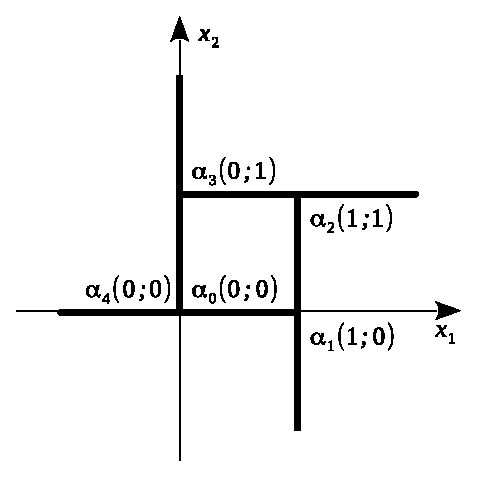
\includegraphics[width=7.5cm]{quad2-2.eps}
	\caption{Отмеченные точки}
	\label{fig:somelabel2}
%\end{figure}
\end{wrapfigure}


\begin{wrapfigure}[14]{r}{7.5cm}
%\begin{figure}
%	%\vspace{-5ex}
	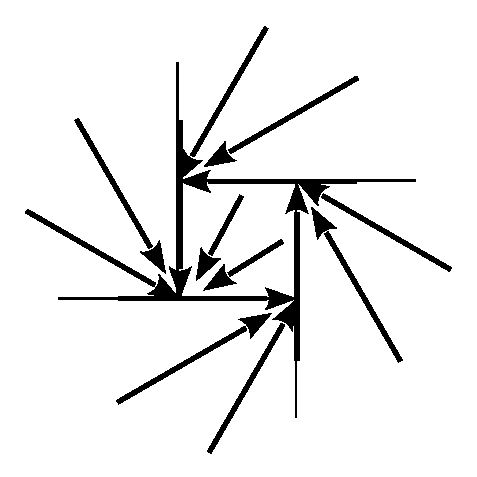
\includegraphics[width=7.5cm]{quad2-3.eps}
	\caption{Направления сдвигов}
	\label{fig:somelabel3}
%\end{figure}
\end{wrapfigure}


\end{document}
